%!TEX root = report.tex
\chapter{Repricer Algorithm}
\label{sec:repricer}

\section{Problem Understading}
\label{sec:rpproblem}

One of the main inputs influencing who becomes the auction winner is the price offered by a seller for the product being auctioned. Product prices change dynamically on the Amazon platform, depending on the real-time competition for selling that product (i.e., the competing offers) and manual repricing rules decided by the seller. We aim to automate the repricing strategy to adapt to observed changes in auction behaviour. The repricing strategy helps to maximise the probability of winning the next auction for the given seller/customer and product. 
 
The problem to be solved is: can we use our BuyBox predictor algorithm to dynamically recommend a product price to a given seller (i.e., a dynamic repricing strategy), for a given auction?

This section provides a dynamic repricing tool that uses BuyBox prediction model in Section \ref{sec:buybox}. The repricing algorithm takes in data describing an auction for a given product and a given seller on the Amazon Marketplace, the BuyBox predictor model trained to predict the winner of any auction (a BuyBox winner predictor algorithm) and the data used to train that model. As output, it produces a few candidate price points for the given customer in the auction, ranks the price candidates and selects the top ranked price as a new price recommendation for that customer.

\section{Spliting the Price's Bins}
\label{sec:spliting}

The first problem we have to solve is how to generate the recommended candidate prices.

\section{Finding Recommendation Score}
\label{sec:finalscore}

\section{Proposed Algorithm for Repricer}

\label{sec:repricermodel}


\begin{figure}[!h]
	\begin{center}
		\scalebox{0.70}{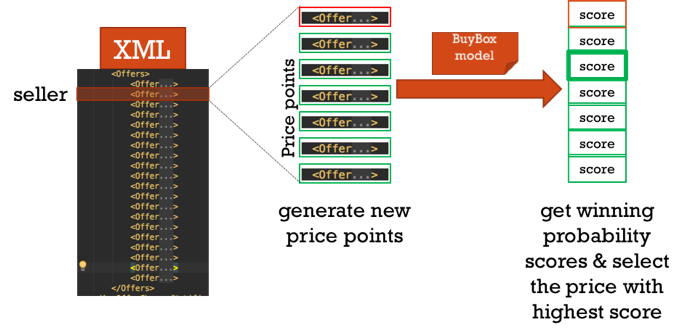
\includegraphics{fig5_repricer.png}}
	\end{center}
	\caption{\label{fig:repricerflow}The flowchart of repricing strategy for one specific seller.
	}
\end{figure}

We provide here the repricing strategy to generate the predictive move of repricing. Our concentration is on the probability of what point of price we can get into buy box with the highest chance we can do. The strategy is defined into three steps:

1) First step is the getting and splitting. We get the point of our customer, who want to make a repricing.
After receive the customer's price, we generate many bins of price, which we would like to test the probability. 

2) Second step is the applying model and generating prediction score. On this step, we apply the Random Forest model, which is learned in BuyBox Predictor. Then we calculate the final scores of all price's points.

3) Final step is selecting. The top 10 largest scores, which has the highest probability to occupy the buy box, is provided as recommended price points. 


\section{Experiment for Repricing}
\label{sec:exprepricer}



\begin{figure}[!h]
	\begin{center}
		\scalebox{0.60}{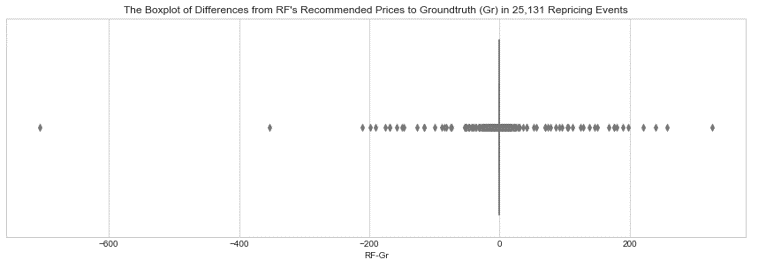
\includegraphics{fig_Boxplot_WinCase.png}}
	\end{center}
	\caption{\label{fig:lostcase}The Box plot of Prediction for Winning Cases.}
\end{figure}


\begin{figure}[!h]
	\begin{center}
		\scalebox{0.60}{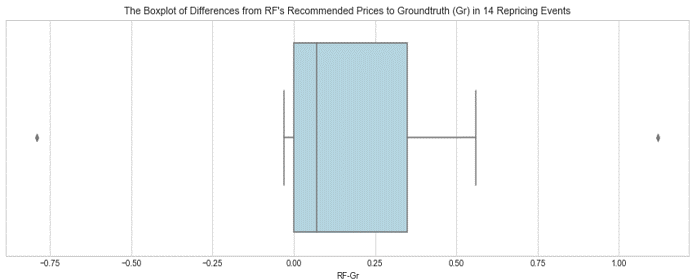
\includegraphics{fig_Boxplot_LostCase.png}}
	\end{center}
	\caption{\label{fig:lostcase}The Box plot of Prediction for Losing Cases.}
\end{figure}